\documentclass[tikz,border=0pt]{standalone}
\usepackage{xcolor}
\usetikzlibrary{calc}
% Palette: Sam_Comm_final.png by eye, and the drones and raiders.
\definecolor{ink}{HTML}{3B2340}
\definecolor{sky}{HTML}{EFC46A}
\definecolor{skyhi}{HTML}{F5DA92}
\definecolor{skylow}{HTML}{E9B060}
\definecolor{cloud}{HTML}{F2D58A}
\definecolor{paper}{HTML}{FBEFD0}
\definecolor{cream}{HTML}{FFF6E0}
\definecolor{white}{HTML}{FFFFFF}
\definecolor{wallA}{HTML}{E88A73}
\definecolor{wallB}{HTML}{EE9F7E}
\definecolor{wallC}{HTML}{E47A7E}
\definecolor{wallD}{HTML}{F0B07E}
\definecolor{wallE}{HTML}{D9765F}
\definecolor{wallF}{HTML}{E99A8A}
\definecolor{greenA}{HTML}{8DBB7E}
\definecolor{greenB}{HTML}{6FA77A}
\definecolor{greenC}{HTML}{A9C97F}
\definecolor{greenD}{HTML}{5E9C6A}
\definecolor{greenE}{HTML}{4A8060}
\definecolor{sage}{HTML}{9DB98A}
\definecolor{sagedark}{HTML}{6F8F66}
\definecolor{sagelight}{HTML}{C2D6A6}
\definecolor{window}{HTML}{F6E7A0}
\definecolor{windark}{HTML}{8C5A64}
\definecolor{metal}{HTML}{8D9A93}
\definecolor{metaldark}{HTML}{5E6B66}
\definecolor{metallight}{HTML}{B9C4BC}
\definecolor{wood}{HTML}{B9835A}
\definecolor{wooddark}{HTML}{8C5A3C}
\definecolor{woodlight}{HTML}{D9A66F}
\definecolor{stone}{HTML}{E7C9A0}
\definecolor{stonedark}{HTML}{C9A47E}
\definecolor{concrete}{HTML}{D8C3A4}
\definecolor{concretedark}{HTML}{B8A084}
\definecolor{asphalt}{HTML}{8E7A86}
\definecolor{asphaltdark}{HTML}{6E5C68}
\definecolor{roadline}{HTML}{F6E7A0}
\definecolor{kerb}{HTML}{D8B48C}
\definecolor{red}{HTML}{E0483E}
\definecolor{redlight}{HTML}{F27A6A}
\definecolor{gold}{HTML}{FFB000}
\definecolor{goldlight}{HTML}{FFD54F}
\definecolor{teal}{HTML}{4FA3A0}
\definecolor{tealdark}{HTML}{3C8582}
\definecolor{magenta}{HTML}{FF2E88}
\definecolor{cyan}{HTML}{13CFE3}
\definecolor{violet}{HTML}{8A5BD6}
\definecolor{orange}{HTML}{F2803A}
\definecolor{pink}{HTML}{F48FB1}
\definecolor{glow}{HTML}{4FE6E0}
\definecolor{glowhi}{HTML}{C8FFF9}
\definecolor{hot}{HTML}{FF6A1A}
\definecolor{hothi}{HTML}{FFD07A}
\definecolor{armour}{HTML}{7E7A86}
\definecolor{armourdark}{HTML}{5A5466}
\definecolor{armourlight}{HTML}{A8A2B0}
\definecolor{wasp}{HTML}{E0A82E}
\definecolor{waspdark}{HTML}{B07E1A}
\definecolor{moth}{HTML}{F2E6C8}
\definecolor{mothdark}{HTML}{D2C09A}
\definecolor{hornet}{HTML}{3C8582}
\definecolor{hornetdark}{HTML}{2C6260}
\definecolor{warden}{HTML}{E47A7E}
\definecolor{wardendark}{HTML}{B85A62}
\definecolor{tick}{HTML}{8DBB7E}
\definecolor{tickdark}{HTML}{5E8A5A}
\definecolor{strider}{HTML}{D9765F}
\definecolor{striderdark}{HTML}{A8543F}
\definecolor{jacket}{HTML}{6FA77A}
\definecolor{jacketb}{HTML}{4FA3A0}
\definecolor{jacketc}{HTML}{E88A73}
\definecolor{jacketd}{HTML}{F0B07E}
\definecolor{skin}{HTML}{F2C49A}
\definecolor{skinb}{HTML}{C98C6A}
\definecolor{skinc}{HTML}{8C5A3C}
\definecolor{hair}{HTML}{3B2340}
\definecolor{goo}{HTML}{B6E35A}
\definecolor{goodark}{HTML}{7FB23A}
\newcommand{\Ink}{1.8pt}
\tikzset{inked/.style={draw=ink, line width=\Ink, line join=round, line cap=round}}
\begin{document}
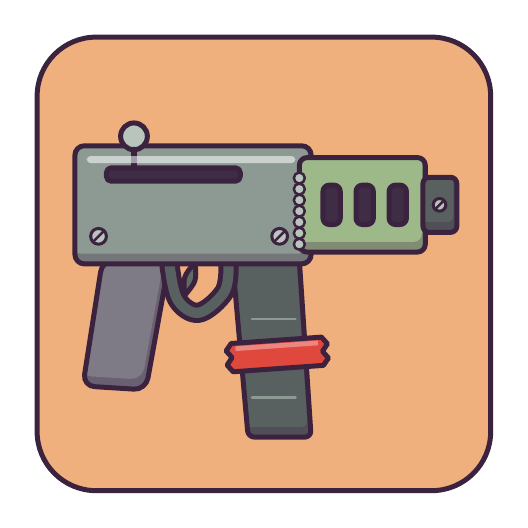
\begin{tikzpicture}
\clip (0,0) rectangle (6,6);
\fill[wallD] [rounded corners=0.75cm] (0.12,0.12) rectangle (5.88,5.88);
\begin{scope}\clip [rounded corners=0.75cm] (0.12,0.12) rectangle (5.88,5.88);
\begin{scope}\clip[rounded corners=0.08cm] (2.6,3.05) -- (3.45,3.05) -- (3.6,0.8) -- (2.8,0.8) -- cycle;
\fill[metaldark!85!ink!70!ink,rounded corners=0.08cm] (2.6,3.05) -- (3.45,3.05) -- (3.6,0.8) -- (2.8,0.8) -- cycle;
\fill[metaldark!85!ink,rounded corners=0.08cm, shift={(-0.045,0.13)}] (2.6,3.05) -- (3.45,3.05) -- (3.6,0.8) -- (2.8,0.8) -- cycle;
\end{scope}
\draw[inked,rounded corners=0.08cm] (2.6,3.05) -- (3.45,3.05) -- (3.6,0.8) -- (2.8,0.8) -- cycle;
\draw[metal, line width=1pt, line cap=round] (2.85,1.3) -- (3.4,1.3);
\draw[metal, line width=1pt, line cap=round] (2.85,1.8) -- (3.4,1.8);
\draw[metal, line width=1pt, line cap=round] (2.85,2.3) -- (3.4,2.3);
\filldraw[inked,fill=red] (2.609,1.63) -- (3.756,1.711) -- (3.82,1.805) -- (3.744,1.89) -- (3.807,1.985) -- (3.731,2.07) -- (2.584,1.989) -- (2.52,1.895) -- (2.596,1.81) -- (2.533,1.715) -- cycle;
\fill[white, opacity=0.35] (2.641,1.893) -- (3.688,1.966) -- (3.684,2.026) -- (2.637,1.953) -- cycle;
\begin{scope}\clip[rounded corners=0.15cm] (0.95,3.05) -- (1.8,3.05) -- (1.5,1.4) -- (0.7,1.45) -- cycle;
\fill[armour!70!ink,rounded corners=0.15cm] (0.95,3.05) -- (1.8,3.05) -- (1.5,1.4) -- (0.7,1.45) -- cycle;
\fill[armour,rounded corners=0.15cm, shift={(-0.045,0.13)}] (0.95,3.05) -- (1.8,3.05) -- (1.5,1.4) -- (0.7,1.45) -- cycle;
\end{scope}
\draw[inked,rounded corners=0.15cm] (0.95,3.05) -- (1.8,3.05) -- (1.5,1.4) -- (0.7,1.45) -- cycle;
\draw[ink, line width=7.299pt, line cap=round, line join=round] plot[smooth, tension=0.6] coordinates {(1.8,3) (1.9,2.55) (2.175,2.38) (2.5,2.65) (2.55,3)};
\draw[metaldark!85!ink, line width=3.699pt, line cap=round, line join=round] plot[smooth, tension=0.6] coordinates {(1.8,3) (1.9,2.55) (2.175,2.38) (2.5,2.65) (2.55,3)};
\filldraw[inked,fill=metaldark] (2.125,3.02) .. controls (2.146,2.783) .. (1.995,2.6) .. controls (1.974,2.837) .. (2.125,3.02) -- cycle;
\begin{scope}\clip[rounded corners=0.12cm] (0.6,3) rectangle (3.6,4.5);
\fill[metal!70!ink,rounded corners=0.12cm] (0.6,3) rectangle (3.6,4.5);
\fill[metal,rounded corners=0.12cm, shift={(-0.045,0.13)}] (0.6,3) rectangle (3.6,4.5);
\end{scope}
\draw[inked,rounded corners=0.12cm] (0.6,3) rectangle (3.6,4.5);
\begin{scope}\clip[rounded corners=0.1cm] (3.45,3.15) rectangle (5.05,4.35);
\fill[sage!70!ink,rounded corners=0.1cm] (3.45,3.15) rectangle (5.05,4.35);
\fill[sage,rounded corners=0.1cm, shift={(-0.045,0.13)}] (3.45,3.15) rectangle (5.05,4.35);
\end{scope}
\draw[inked,rounded corners=0.1cm] (3.45,3.15) rectangle (5.05,4.35);
\begin{scope}\clip[rounded corners=0.08cm] (3.75,3.5) rectangle (3.97,4);
\fill[ink!88!metaldark!70!ink,rounded corners=0.08cm] (3.75,3.5) rectangle (3.97,4);
\fill[ink!88!metaldark,rounded corners=0.08cm, shift={(0,0)}] (3.75,3.5) rectangle (3.97,4);
\end{scope}
\draw[inked,rounded corners=0.08cm] (3.75,3.5) rectangle (3.97,4);
\begin{scope}\clip[rounded corners=0.08cm] (4.17,3.5) rectangle (4.39,4);
\fill[ink!88!metaldark!70!ink,rounded corners=0.08cm] (4.17,3.5) rectangle (4.39,4);
\fill[ink!88!metaldark,rounded corners=0.08cm, shift={(0,0)}] (4.17,3.5) rectangle (4.39,4);
\end{scope}
\draw[inked,rounded corners=0.08cm] (4.17,3.5) rectangle (4.39,4);
\begin{scope}\clip[rounded corners=0.08cm] (4.59,3.5) rectangle (4.81,4);
\fill[ink!88!metaldark!70!ink,rounded corners=0.08cm] (4.59,3.5) rectangle (4.81,4);
\fill[ink!88!metaldark,rounded corners=0.08cm, shift={(0,0)}] (4.59,3.5) rectangle (4.81,4);
\end{scope}
\draw[inked,rounded corners=0.08cm] (4.59,3.5) rectangle (4.81,4);
\filldraw[inked,fill=metallight,line width=0.9pt] (3.45,3.25) circle (0.07);
\filldraw[inked,fill=metallight,line width=0.9pt] (3.45,3.39) circle (0.07);
\filldraw[inked,fill=metallight,line width=0.9pt] (3.45,3.53) circle (0.07);
\filldraw[inked,fill=metallight,line width=0.9pt] (3.45,3.67) circle (0.07);
\filldraw[inked,fill=metallight,line width=0.9pt] (3.45,3.81) circle (0.07);
\filldraw[inked,fill=metallight,line width=0.9pt] (3.45,3.95) circle (0.07);
\filldraw[inked,fill=metallight,line width=0.9pt] (3.45,4.09) circle (0.07);
\begin{scope}\clip[rounded corners=0.06cm] (1,4.05) rectangle (2.7,4.22);
\fill[ink!88!metaldark!70!ink,rounded corners=0.06cm] (1,4.05) rectangle (2.7,4.22);
\fill[ink!88!metaldark,rounded corners=0.06cm, shift={(0,0)}] (1,4.05) rectangle (2.7,4.22);
\end{scope}
\draw[inked,rounded corners=0.06cm] (1,4.05) rectangle (2.7,4.22);
\filldraw[inked,fill=metallight] (1.35,4.62) circle (0.17);
\draw[ink, line width=2.2pt, line cap=round] (1.35,4.45) -- (1.35,4.22);
\fill[white, opacity=0.55, rounded corners=0.05cm] (0.75,4.28) rectangle (3.4,4.37);
\filldraw[inked,fill=metallight,line width=1.1pt] (0.9,3.35) circle (0.1);
\draw[ink, line width=0.9pt, line cap=round] (0.845,3.295) -- (0.955,3.405);
\filldraw[inked,fill=metallight,line width=1.1pt] (3.2,3.35) circle (0.1);
\draw[ink, line width=0.9pt, line cap=round] (3.145,3.295) -- (3.255,3.405);
\begin{scope}\clip[rounded corners=0.08cm] (5.02,3.4) rectangle (5.45,4.1);
\fill[metaldark!85!ink!70!ink,rounded corners=0.08cm] (5.02,3.4) rectangle (5.45,4.1);
\fill[metaldark!85!ink,rounded corners=0.08cm, shift={(-0.045,0.13)}] (5.02,3.4) rectangle (5.45,4.1);
\end{scope}
\draw[inked,rounded corners=0.08cm] (5.02,3.4) rectangle (5.45,4.1);
\filldraw[inked,fill=metallight,line width=1.1pt] (5.23,3.75) circle (0.08);
\draw[ink, line width=0.9pt, line cap=round] (5.186,3.706) -- (5.274,3.794);
\end{scope}
\draw[inked] [rounded corners=0.75cm] (0.12,0.12) rectangle (5.88,5.88);
\end{tikzpicture}
\end{document}
